% 
% Chickens, Anyone?  (BOOK version)
% (c) 2009 Eric R. Jeschke (eric@redskieatnight.com).
% This work is licensed under a Creative Commons Attribution-Share Alike
% 3.0 United States License
% See http://creativecommons.org/licenses/by-sa/3.0/us/
%
% Eric Jeschke makes no representation about the suitability or accuracy
% of this software or data for any purpose, and makes no warranties,
% either express or implied, including merchantability and fitness for a
% particular purpose or that the use of this software or data will not
% infringe any third party patents, copyrights, trademarks, or other
% rights.  The software and data are provided "as is". 
%
% 
% If you make a .sty file, please let me know!
%
% [top-level file]
\nonstopmode

\documentclass[10pt,final,openany]{book}
\usepackage{graphicx}
% where can I find the photos that will be imported for this version
\graphicspath{{./photos.book/}}

% font configuration is factored out
% Only uncomment if you have the fontspec package installed
% You will have to set the appropriate font names for what you have
% installed.
%
% You might be able to use opentype tools to find out the names of
% the fonts you can use here, or you can just experiment
%  $ otfinfo -a .../*.ttf
%
\usepackage{fontspec}
\setmainfont[
    Mapping=tex-text,
    ItalicFont={EBGaramond12-Italic.otf}
]{EBGaramond12-Regular.otf}
\setsansfont[Mapping=tex-text]{Arial}
\setmonofont[Mapping=tex-text]{Courier New}


% in case you want to embed any hyperlinks
% turn on colorlinks to avoid the nasty box around the link
\usepackage[colorlinks=true,urlcolor=black]{hyperref}

% geometry package is a much more reasonable way to set margins in LaTeX
% for Blurb, set this to the actual desired size as indicated by the
% size calculator on their web site
\usepackage[paperwidth=9.625in, paperheight=8.25in, 
            % amount we 'lose' (visually) due to the binding
            % left and right pages are offset a bit to the sides
            % (typically looks better for most kinds of bindings)
            bindingoffset=0.25in,
            % set total to the dimensions of the printed part
            total={8in,7.75in},
            % include header/footer/margin notes in printed area
            twoside, includeall, nomarginpar,
            ignorehead=false, ignorefoot=false, ignoremp=false,
            % center printed area on page
            vcentering, hcentering]{geometry}

% only play with these if you are going to do margin notes
% width of margin notes area
%\setlength{\marginparwidth}{0in}
% distance between margin and paragraph
%\setlength{\marginparsep}{0in}

% footer configuration 
\setlength{\footnotesep}{10pt}

% header configuration
\setlength{\headheight}{10pt}
\setlength{\headsep}{0.1in}

\title{Chickens, Anyone?}
\author{Eric Jeschke}

%%%%%%%%% PDF/X-3 stuff, necessary for Blurb IF USING pdflatex %%%%%%%%%
% ICC color profiles are embedded in the images
%% \pdfinfo{
%% /Title (Chickens, Anyone?)   % set your title here
%% /Author (Eric Jeschke)       % set author name
%% /Subject (Chickens)          % set subject
%% /Keywords (Chickens, Hawaii) % set keywords
%% /Trapped (False)
%% /GTS_PDFXVersion (PDF/X-3:2002)
%% }
%% % must have a trim box, but I think Blurb ignores the values
%% \pdfpageattr{%/MediaBox [0 0 693.36000 594.00000]
%% /TrimBox [0.00000 9.00000 684.36000 585.00000]}
%% \pdfminorversion=3
%% \pdfcatalog{
%% /OutputIntents [ <<
%% /Info (none)
%% /Type /OutputIntent
%% /S /GTS_PDFX
%% /OutputConditionIdentifier (Blurb.com)
%% /RegistryName (http://www.color.org/)
%% >> ]
%% }

%%%%%%%%% PDF/X-3 stuff, necessary for Blurb IF USING xelatex %%%%%%%%%
\special{pdf:docinfo <<
/Title (Chickens, Anyone?)   % set your title here
/Author (Eric Jeschke)       % set author name
/Subject (Chickens)          % set subject
/Keywords (Chickens, Hawaii) % set keywords
/Trapped (False)
/GTS_PDFXVersion (PDF/X-3:2002)
% must have a trim box, but I think Blurb ignores the values
/TrimBox [0.00000 9.00000 684.36000 585.00000] >>
}
\special{pdf:put @catalog <<
/OutputIntents [ <<
/Info (none)
/Type /OutputIntent
/S /GTS_PDFX
/OutputConditionIdentifier (Blurb.com)
/RegistryName (http://www.color.org/)
>> ] >>
}

% paragraph indentations
\setlength{\parindent}{0in}
% amount of space before each new paragraph begins
\setlength{\parskip}{1em}
    

% comment to force even justification
\raggedright

\begin{document}

\pagestyle{empty}

% bring in the rest of the content which is in common with the book
% version
%
% common information to the web version and book version
%
% images will be imported by searching the paths set with \graphicspath
% the book.tex or web.tex sets this so the correct resolution images end
% up in the correct document.
% 
% cover is done elsewhere, as this is usually broken out from the 
% ``text block'' for POD publishing--see book.tex
%
\newcommand{\signed}[1]{\par\hfill\normalfont--- \textit{#1}}

\newpage

\vspace*{1in}
\begin{center}
{\Large from the Carpentries} 

{\LARGE for Greg}

{\large (who would have `enjoyed' typesetting this book)}

\vspace*{0.5in}

\includegraphics[width=3in]{gregwilson}
\end{center}
\newpage

\vspace*{1in}
{\LARGE About this book}

% TODO: Some brief introductory text here

\newpage
% Blake Stamps

Greg taught my SWC instructor training course via teleconference in 2015. Even
though I met him through a screen his ability to convey what it is to really
teach, and the passion by which he conveyed his message really stuck with me.
I've carried that on through my postdoc, and I just wanted to say thank you
Greg.

\signed{Blake Stamps}

\newpage
% Shoaib Sufi

I was inspired by your drive to do what you thought was best and right in your
career (University of Toronto) and due to human factors (Mozilla Science Lab)
at work. Seeing professional integrity in action is different than reading it
from a book. Also, I won't forget your railing against too many workshops
covering the same ground at the Software Credit Workshop
(www.software.ac.uk/software-credit) while highlighting your research around
teaching software skills being the only sustainable approach to improve
practice; I liked the combination of critique and imparting actionable
knowledge. I still don't know why you hate Git so much, but if there is a blog
post about this, then do send me the link, I am sure it's well founded  :  D  -
All the best in your future endeavours and to your family! 

\signed{Shoaib Sufi}

\newpage
% Gang Liu

I was ever trained in his course for lectures of the software carpentry. I was
deeply impressed by his passionate enthusiasm. It will be a big loss to the
software carpentry when he leaves. Hope Greg have a wonderful future and the
software carpentry still be good.

\signed{Gang Liu}

\newpage

\newpage
% Timothée Poisot

Greg, the instructor training changed my life. At least the part of it spent
teaching. You are a folk hero in the lab, and all the students around realise
how much Software Carpentry changed the way we can immerse ourselves in
computing. Thank you!

\signed{Timoth\'{e}e Poisot}

\newpage
% Auriel Fournier

When I first started instructor training I was nervous, since most of my
interactions with people who code hadn't been positive. Greg's warmth, care and
welcoming attitude quickly endeared me to him and the whole carpentry
community. He took an interest in me as a person and has been a huge
inspiration to me on how to approach science, teaching, and life. 

\signed{Auriel Fournier}

\newpage
\pagestyle{plain}
% Russell Alleen-Willems
\begin{minipage}{0.45\textwidth}
    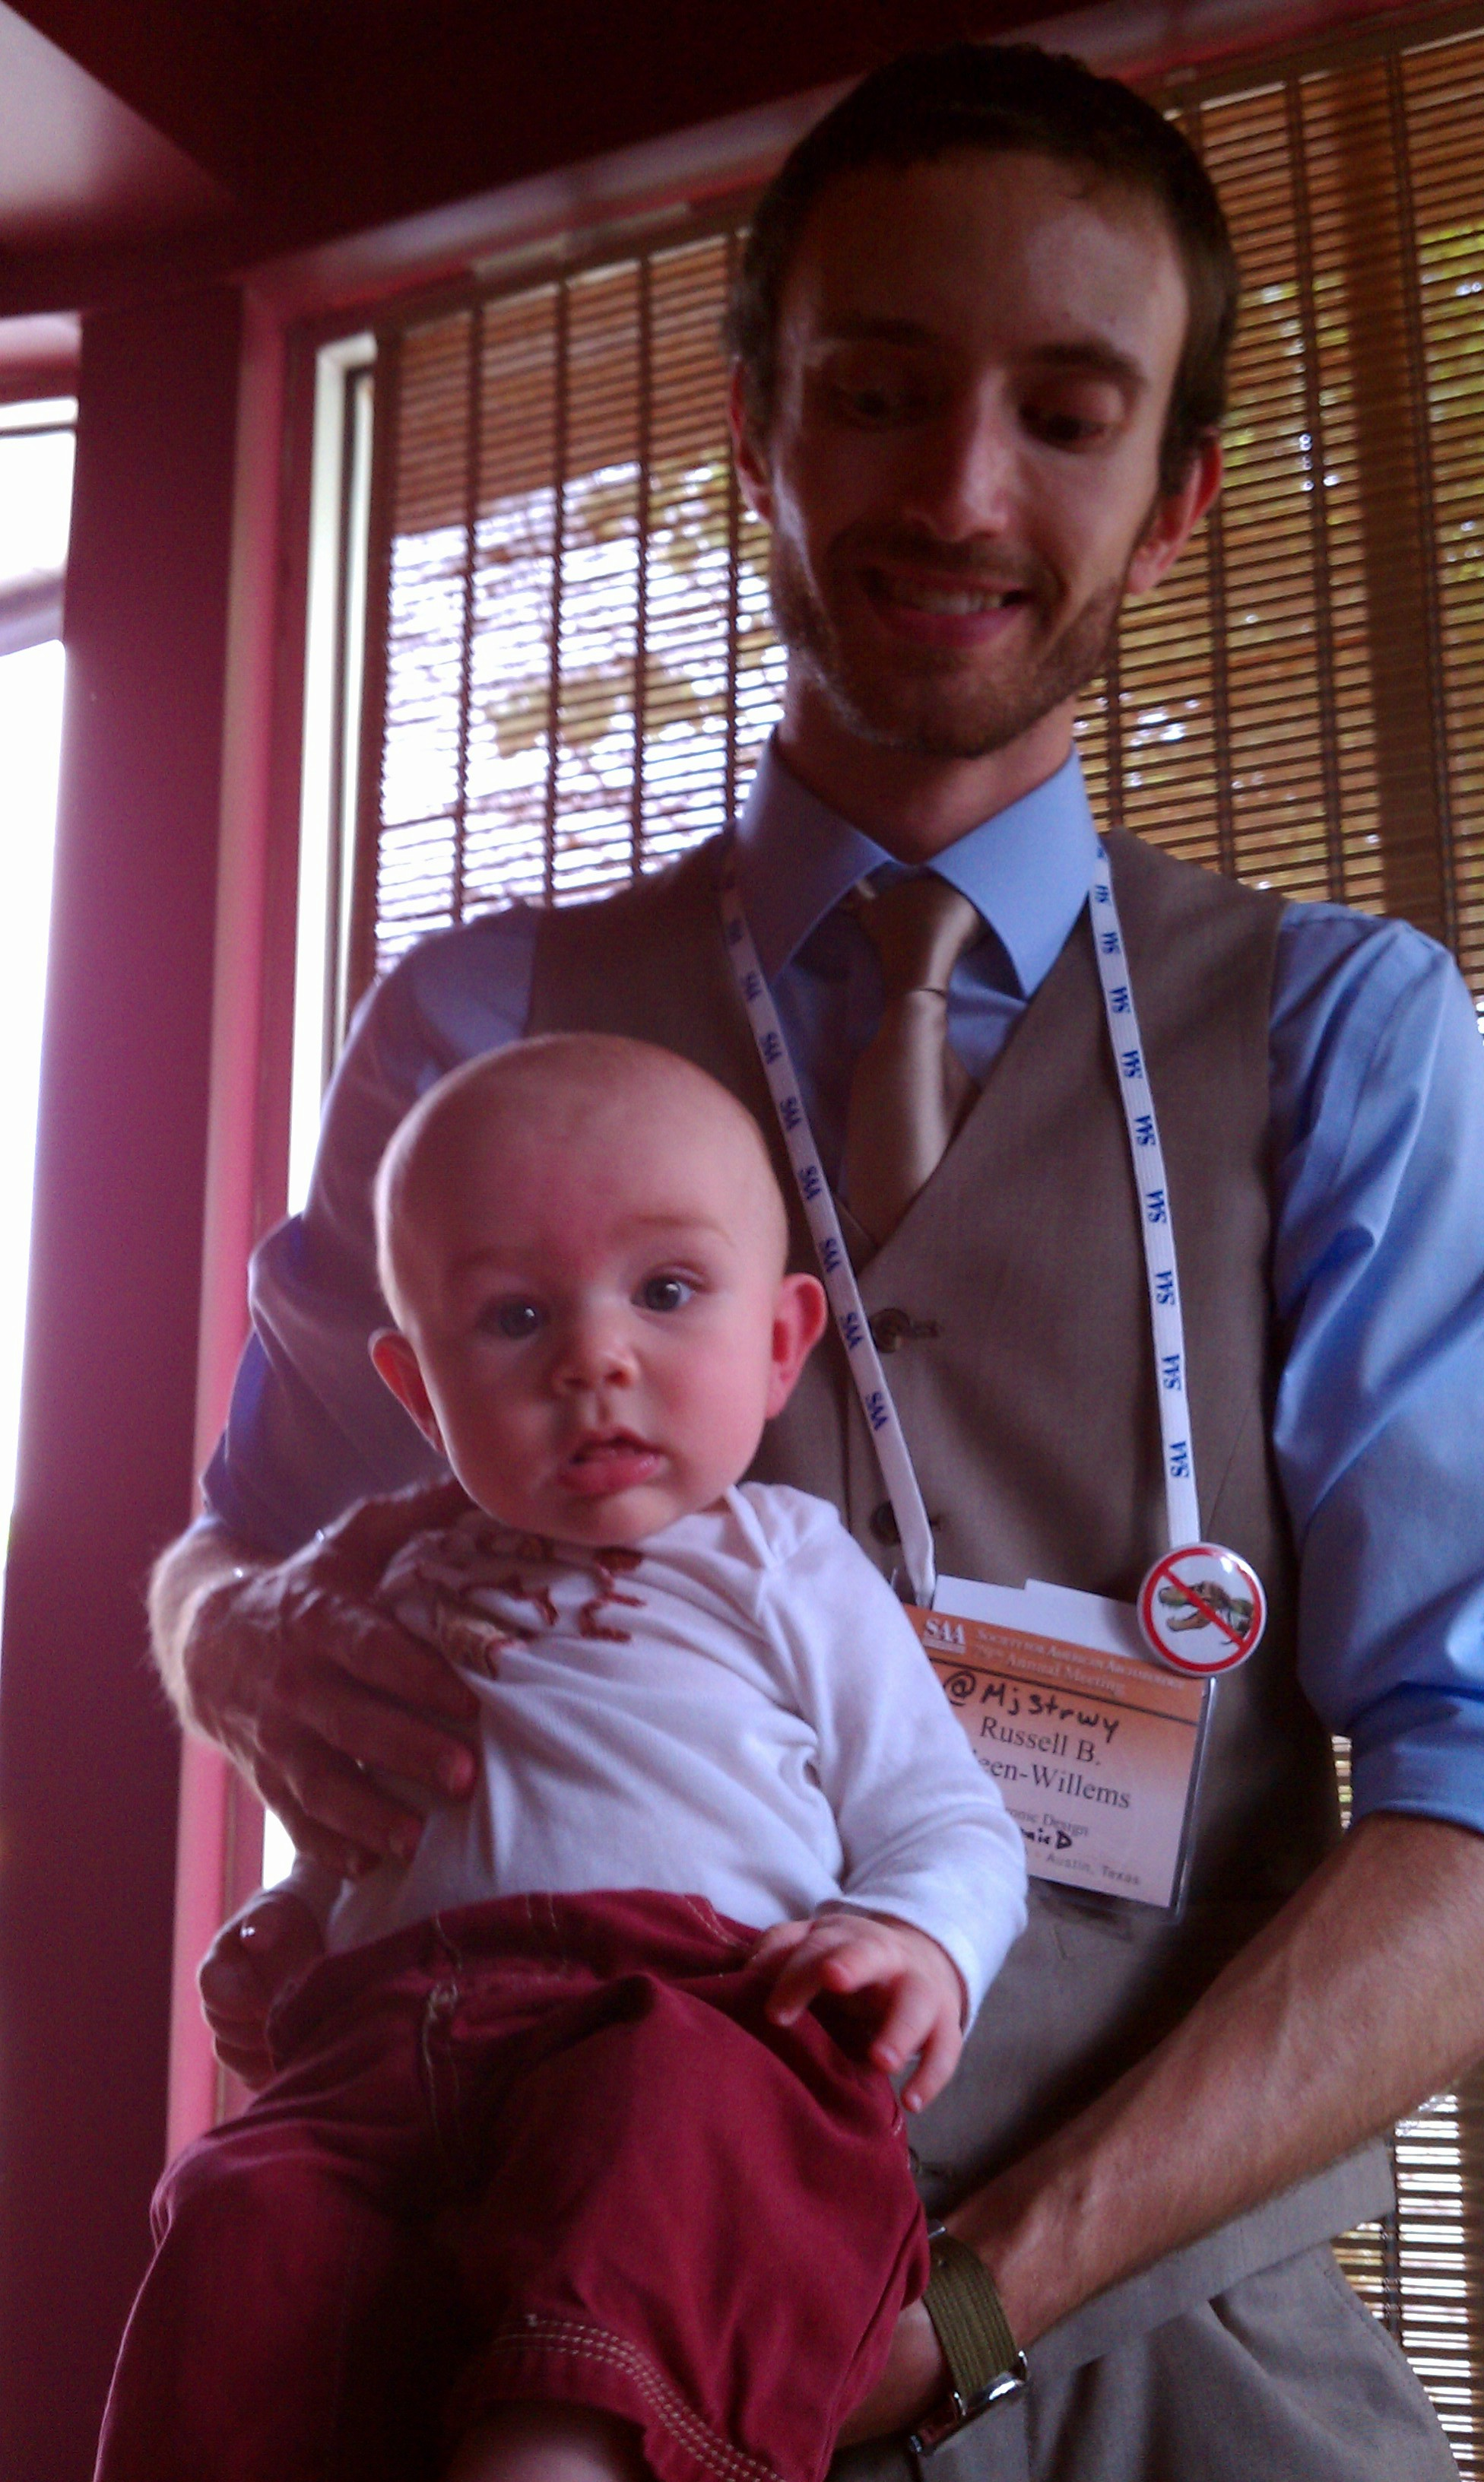
\includegraphics[width=3in]{russell}
\end{minipage}
\hfill
\begin{minipage}{0.45\textwidth}
\setlength{\parindent}{0in}
\setlength{\parskip}{1em}
I first met Greg during the 2014 Software Carpentry Instructor Training he held
online. I was a stay at home dad at the time and split my time between work
projects and watching my newborn son, Nova. Often I would have to attend
the SWC training sessions with my son napping in his baby carrier strapped
to my chest. Nova slept pretty well, and I tried to make judicious use of
the mute button so the session wasn't filled with baby noises. 

Greg, as a father himself, not only tolerated my son being in class with
me, but even seemed happy that he was there. Sometimes Greg also had to
teach with his daughter in tow if she was home ill. It was good for me to
see Greg model how being a scientist and active leader can mesh with the
other important roles in our lives. 

Thanks for all your hard work Greg, and best of luck in your future endeavors! 

[Photo is of me at the Society for American Archaeology conference with my son
in tow. I couldn't find a good picture of me and Nova at a SWC session, either
remote or in-person]

\signed{Russell Allen-Willems}
\end{minipage}

\newpage
% James Hetherington

Greg's sense of mission, his commitment to the importance of readability and
reproducibility in scientific software, were hugely important to my focus and
confidence in contributing to the Research Software Engineering movement in the
UK. His advice and support have been important on many occasions in the story
of the UCL research software group.

I remember at Sci Py going swimming at Barton Springs Pool with a number of
research software heros, including Greg and Fernando Perez. One of those weird
moments when you find yourself socialising at a peer level with people who were
once legends! I've been an admirer of Greg's at least since \title{Beautiful
Code}.

Another moment characteristic of Greg's considerateness: I remember Greg moving
aside to the other room when we taught carpentry together the first time in
Greenwich: to make sure my teaching wasn't worsened by being starstruck! A big
vote of confidence that meant a lot.

\signed{James Hetherington}

\newpage
% Rochelle Terman

The first time I met Greg was at UC Berkeley. I was struck by his warmth and
openness. I was a stranger, and he had a busy schedule, and yet he took the
time to sit down with me and have a genuine conversation about SC, pedagogy,
and the future of the classroom. It was at that time that I knew SC was the
right community for me.

\signed{Rochelle Terman}

\newpage
% Madeleine Bonsma
Greg, I will be forever grateful to you for encouraging me and UofT Coders to
hold workshops in Toronto. Thank you for sharing your expertise with us during
instructor training as well. Organizing and leading Software Carpentry
workshops is something I feel so lucky to be able to do, and it's all thanks to
you!

\signed{Madeleine Bonsma}

\newpage
% Raniere Silva

On behalf of all the learners from the workshops in Brazil, ``Thanks very much
for your services.''

\signed{Raniere Silva}

\newpage
% Jessica Gallinger

Thank you for encouraging me to become an instructor and gain confidence in my
skills. It made a difference in my life.

\signed{Jessica Gallinger}

\newpage
% Karthik Srinivasan

Greg is a great instructor and leader. The instructor session was very
interesting. His style of conveying the concepts is inspiring.

\signed{Karthik Srinivasan}

\newpage
% Matt Dickenson

My fondest memory of Greg is receiving my SWC instructor training certificate
with the words ``I believe this is yours.'' Greg, you have had a profound
impact on our community and served as a role model for a generation of
educators.  Thank you and good luck with what's next!

\signed{Matt Dickenson}

\newpage
% Radovan Bast

The Software Carpentry instructor training which I was fortunate to participate
in 2014 has not only profoundly changed the way I prepare and deliver courses
but also changed my career path towards teaching software development tools and
techniques. I still remember every anecdote that Greg has shared with us during
the training. When I prepare new material, I automatically analyze the new
material with Greg's words of advice resonating in my head. Thanks to Greg I
have embraced the importance of exercises and interaction and the importance to
simplify and distill the essence of a course and always mind the cognitive
load. I am very grateful for this experience and wish you all the best for the
future!

\signed{Radovan Bast}

\newpage
% Victor Lee

We, Koreans, appreciate your works. Without your contributions, we would have
hard time to cope with Alpha-Go shock and the fourth industrial revolution.
Now, I am working at one of the president candidates camp as a data scientist.
If he is elected as a ``REAL'' president near future, I'd like to invite you
and have not a Skype meeting, but a real face-to-face meeting. Thanks again. 

\signed{Victor Lee}

\newpage
% Kunal Marwaha

After the instructor training, several of us learners took the bus back with
Greg to Berkeley's campus. Greg was trying to find his way to his next meeting
(at the Berkeley Institute of Data Science); I offered to walk him there. We
got off the bus and approached the streetcorner. The light was red, but I began
walking, motioning for Greg to follow. He wouldn't budge. I turned back,
waiting with him until the light was green. He looked at me and said, ``There's
a fundamental shift in the way you live when you're responsible for someone
else's life. If I had broken my leg just now, who would take care of my
mother?''

Of course this is poorly quoted, but I will remember that lesson most of all.
Thank you, Greg. You are one of my heroes.

\signed{Kunal Marwaha}

\newpage
% Naudene Maree

\begin{center}
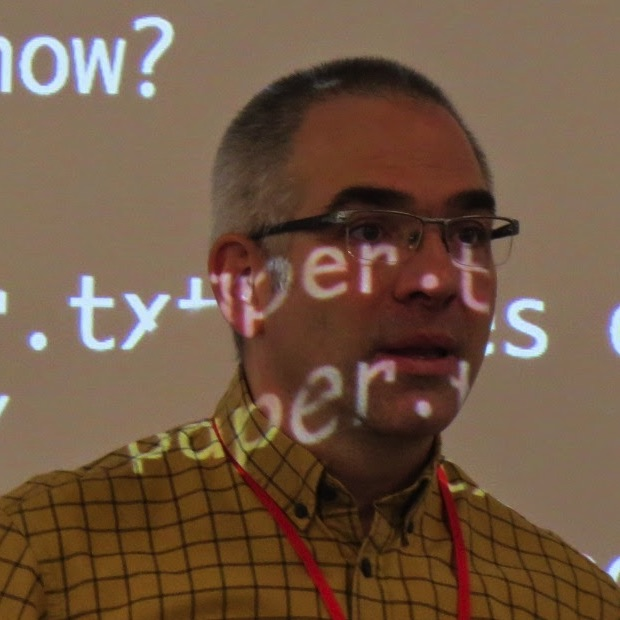
\includegraphics[width=4in]{gvwilson-tgac-large}
\end{center}

My first email from Software Carpentry was an instant reply and I remember
think it must be a computer programmed instant reply. When I asked my check out
helper he simply laughed and replied: ``You could call Greg that''. 

Thanks for make everything run smoothly Mister Computer.

\signed{Naudene Maree}

\newpage
% Kari L. Jordan

In the short time I've known Greg he's encouraged me so much. His knowledge is
undeniable. I am blessed to have been able to work with him, and I hope I can
do my part to continue his legacy.

\signed{Kari L. Jordan}

\newpage
% Adina

My first SWC workshop (bootcamp at the time) teaching experience was a
disaster.  Greg through me into discussing python lists, on what I felt like
was a bit of a whim.  I was totally unprepared and it showed!  I remember
talking to Greg about quitting my teaching ambitions.  After several kind words
of encouragement, his therapy was to make me teach half the next day instead,
it was still pretty disastrous but Greg kept inviting me to teach with him.
And it did get better...so much so that I do it for a living now.  I'll always
remember Greg's discussion on triumph and think of it often on bad teaching
days. 

\signed{Adina}

\newpage
% Abraham Flaxman

Greg Wilson's influence has filtered so deeply into my approach to teaching and
science communication that it is hard to name.  It reminds me of the fish that
does not know it is wet.  Books that his Software Carpentry Train-the-trainers
led me to are now the foundation for my approach to teaching.  I just finished
reading a treatise on standup comedy that I must have heard about from him.
This Thursday I'll teach the second half of the Software Carpentry Python
module, and to prepare I ask myself ``what did Greg do?'' Thank you for your
influential work!

\signed{Abraham Flaxman, University of Washington}

\newpage
% Neal Davis

While I've always appreciated the time Greg has made for face-to-skype time and
mentoring, my favorite experience was the long walk we took through Toronto one
evening post-training.  The reading recommendations you made in that bookstore
were spot-on.  Thanks, Greg--SWC has changed my professional career and I always
be in your debt for that.

\signed{Neal Davis}

\newpage
% Rachel Slaybaugh

You not only inspired me to be a better computational scientist, you inspired
me to teach others to be better computational scientists. You've given me the
tools and approaches to help so many more researchers do reproducible and
transparent research. The ripples will keep going... The impact you have made
on scientific integrity is astonishing. Thank you, truly, for your thought
leadership and for using your actions to fulfill the vision you have for the
world. 

\signed{Rachel Slaybaugh}

\newpage
% Thomas

I came all the way to Montreal for one of the very first SWC workshops aimed at
librarians that you put together, prompted by a tweet and not much thinking.
Within minutes of watching you teach, I knew there was something special there.
You were demystifying something without dumbing it down, with an intense
respect for learners. This made me question most of what I thought about
teaching tech, unlearn what I thought I knew. I'm very fortunate I was able to
complete instructor training with you and I hope I am now approaching all
instances in which I have to teach something to someone with the care and
respect you taught me. Live long and prosper.

\signed{Thomas}

\newpage
% Neem Serra

When I first met you in East Lansing, you told me that I was ``bright but
unfocused.''  You definitely weren't wrong, and I definitely was very annoyed!
Alas, that Software Carpentry workshop and my want to prove that I could be
focused led me down an unexpected path of becoming a software developer.  I
absolutely love it, and I love teaching it to others.  I couldn't have found
myself so truly if it weren't for you, and I'm forever grateful.

\signed{Neem Serra}

\newpage
% Adam Obeng

I learnt a very valuable lesson about teaching when you lead an SWC workshop in
my first year at Columbia.  You masterfully re-directed my smart-ass energy by
foretelling that I would become an instructor. You also gave me a phrase which
has made its way into pretty much all of my talks, classes and projects ever
since: ``Do you want your results to be correct, or just plausible?'' Thank
you!

\signed{Adam Obeng}

\newpage
% Carole Goble
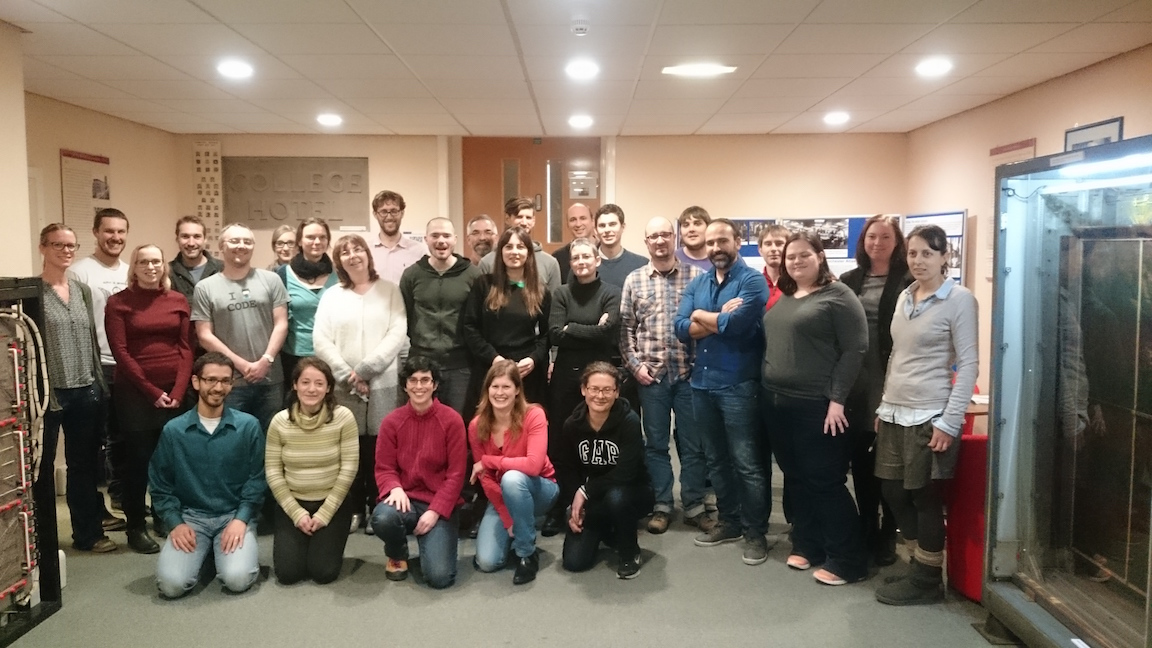
\includegraphics[width=8in]{carole-Instructor-Training-Manchester-2015-11-23}

I met Greg at  a conference in Chicago back in 2012. He was already a legend
and I was apprehensive - what could I do to help him with his mission? As part
of the Software Sustainability Institute, we were already working with Software
Carpentry. He was so inspirational, with such clarity of vision and passion. He
preached. I was blown away.  Meeting with Greg was like meeting with a force of
nature. From then on I was kind of working for him - helping set up SC across
the EU Life Science community through the ELIXIR programme and brokering
sponsorship deals and just doing my best  to promote SC. At a train the
trainers workshop in Manchester late 2015, I had the pleasure of seeing him in
action - handing on the wisdom. He challenged lazy thinking and easy practices,
and showed alternatives. Greg, you are one of the people who I can genuinely
say changed me. May you continue onwards and upwards.

\signed{Carole Goble}

\newpage
% Tommy Guy

If you throw a dart at a globe and hit land, you'll find one of Greg's friends.
If you travel there, you can expect an introduction. He wants his friends to be
friends: that's how he builds a community.

Greg Wilson was the sixth person I met by name in Toronto. He gave me a job
(yep, paid!) TAing for Software Carpentry and building content back when it was
a full semester class and we were producing PowerPoint+video lectures. What
struck me about Greg was his ability to maintain a mission and iterate until he
found the right community. Occasionally, when we were out of money and unsure
where we would get more, the whole thing felt a little Quixotic. Somehow Greg
would mine his legendary breadth of contacts, sell the right people on his
passionately held beliefs, and try again with a new iteration. 

Today, Software Carpentry's global scale, the hundreds of volunteers, the
thousands of students are all the offshoot of a passionate, dogged pursuit of
Greg's original mission to build a community of educators and scientists.

\signed{Tommy Guy}

\newpage
% Chris Medrela

Hi, Greg! I'd like to thank you for all your work at Software Carpentry. Thanks
to that, I found even more joy in my life--SWC helped me discover new hobby,
that is teaching and conducting workshops. Also, before working on AMY, I
didn't know how important it is for my own fulfillment to work on something
that matters, is used and makes difference. Thank you once again and good luck
at Shopify!

\signed{Chris Medrela}

\newpage
% Dan McCloy

The workshop I took from Greg in 2012 was billed as a ``python bootcamp,'' but
it was so much more than that.  It revolutionized how I use computers and how I
think about my day-to-day practice of science.  Five years later, I'm still
learning new things from my memories of what he said.  Having taught a couple
SWC sessions myself recently, I'm also in awe of how efficient he was as a
teacher...  if only my examples and anecdotes were half as memorable as his.

\signed{Dan McCloy}

\newpage
% Marc Sze

Greg, although we only met for a short period in person, you have had a huge
impact on the way that I approach teaching.  I thoroughly enjoyed your stories
during instructor training and really appreciated your opinions when you
visited the University of Michigan in 2016.  If I can express, both for my
research area and teaching, only half of the energy and passion that you have I
will consider myself a success.  Good luck with your future endeavors, you will
most definitely be missed and hard to replace within the Software Carpentry
ecosystem.     

\signed{Marc Sze}

\newpage
% Paul Wilson

I discovered Greg quite by accident in the form of his 2006 presentation at
Purdue university (https://nanohub.org/resources/1811).  I can't remember
exactly what year it was and what series of searches and hyperlinks caused me
to land there, but my approach to research has not been the same since.  I
immediately showed the video to my research group, did a one day in-service to
begin training them with the few relevant skills that I had.  This ultimately
inspired The Hacker Within [THW], my students started to train me, and it all
came full circle when THW invited Greg to visit Madison, WI, as the keynote for
our first Software Carpentry Workshop in January 2011. Six years later,
Software Carpentry lessons are required reading when joining my group, many of
my students become trained instructors, and our campus trains about 150
learners a year in regular Carpentry workshops.  Greg has left an indelible
mark on me, those who pass through my group, and my research.

\signed{Paul Wilson}

\newpage
% Jessica Upani

Greg you are special to me. I was a new comer to Software Carpentry when I met
you. I had no knowledge of GitHub, nor did I know what to expect when I had to
do my teaching demo. Everything was scary to me at that time, but you walked me
through each step patiently successfully. I was the happiest girl when you
wrote me an email title ``I believe this is yours!''. I will forever be
grateful for your kindness. Fly higher in your new journey and always be a
WINNER. Thank you!

\signed{Jessica Upani}

\newpage
% Jessica Mizzi

The first time I took a Train the Trainers course with Greg I was struck by his
enthusiasm for pedagogy. After contributing to SWC online materials, teaching
my first workshop, and helping out with other workshops, I helped out with
another Train the Trainers session. The learners in that session were
captivated by Greg's instruction, just as I was the first time witnessing his
instruction, as evident from the sticky note feedback after the workshop. I
feel lucky to have worked with Greg, and I look forward to continuing
involvement with this great organization that he has built.

\signed{Jessica Mizzi}

\newpage
% Ethan White

During the morning coffee break at the first workshop I ever taught with Greg
he was chatting with some of the students who told him they were interested in
seeing reproducible data analysis in action. At the end of the break he tracks
me down and says ``Hey Ethan, can you do a quick demonstration of some data
analysis in an IPython Notebook if I end 30 minutes early?''. I told him I
didn't have anything prepared, but he told me that whatever I pulled together
in the next hour would be fine, and ran off to teach before I could say no. So,
I sat in the back of the room, sketched something out, gave a live demo of it
without practicing, and it was a huge hit.

This experience taught me that I was capable of using live unrehersed coding as
a teaching technique and that it would be a very powerful one in the right
circumstances. I now regularly use this technique in cases where students want
to learn more about something I haven't planned to cover. I would have never
had the confidence to do this without being pushed into it and my students
regularly say that those sections end up being some of the most valuable
portions of the course. I suspect a lot of folks have similar stories of Greg
pushing them out of their comfort zones in a way that made them better teachers
and scholars. Thanks Greg.

\signed{Ethan White}

\newpage
% Carlos Martinez

Three stone masons were working on a cathedral when someone asked them what
they were doing:

\begin{itemize}
\item ``I am laying bricks'' said the first.
\item ``I am building a wall'' said the second.
\item The third one answered: ``I am constructing the house of God''.
\end{itemize}

Greg inspires people to think that way: not only to see the bigger picture of
what we are doing, but to have a vision of why we are doing what we are doing.

\signed{Carlos Martinez}

\newpage
% Emily Davenport

Greg has a unique gift for community building. When I joined Software Carpentry
as an instructor, Greg reached out personally to each and every person in my
online instructor training cohort, finding out their background, what their
passions were, and how the SWC community to contribute to their personal goals.
The organization's global, diverse perspective is a testament to those efforts.
Thank you Greg, for setting the bar so high and for all that you've done for
the Carpentries.

\signed{Emily Davenport}

\newpage
% Kally Chung

Hi Greg. I had a pleasure to talk with you in Toronto in a cafeteria in front
of Bata Shoe Museum. It was my first trip, and I was alone... Maybe for you it
was only a chat, but you helped me a lot. Your advises, the stories that we
shared... I don't have words to describe how special was this moment for me. 

Well, I'm very happy that you found this special opportunity to explore and I'm
sure that you'll be successful once again. I hope I can have another
opportunity to meet with you and share new stories about teaching and learning.

\signed{Kally Chung}

\newpage
% Scott Chamberlain

I remember the first time I saw Greg teaching - it was a shell lesson at a SWC
workshop in Vancouver. It's not hyperbole when I say I was amazed how good his
lesson was. The academic community is forever indebted to what Greg started
with SWC. 

\signed{Scott Chamberlain}

\newpage
% Ian Hawke
\begin{figure}[h!]
\centering
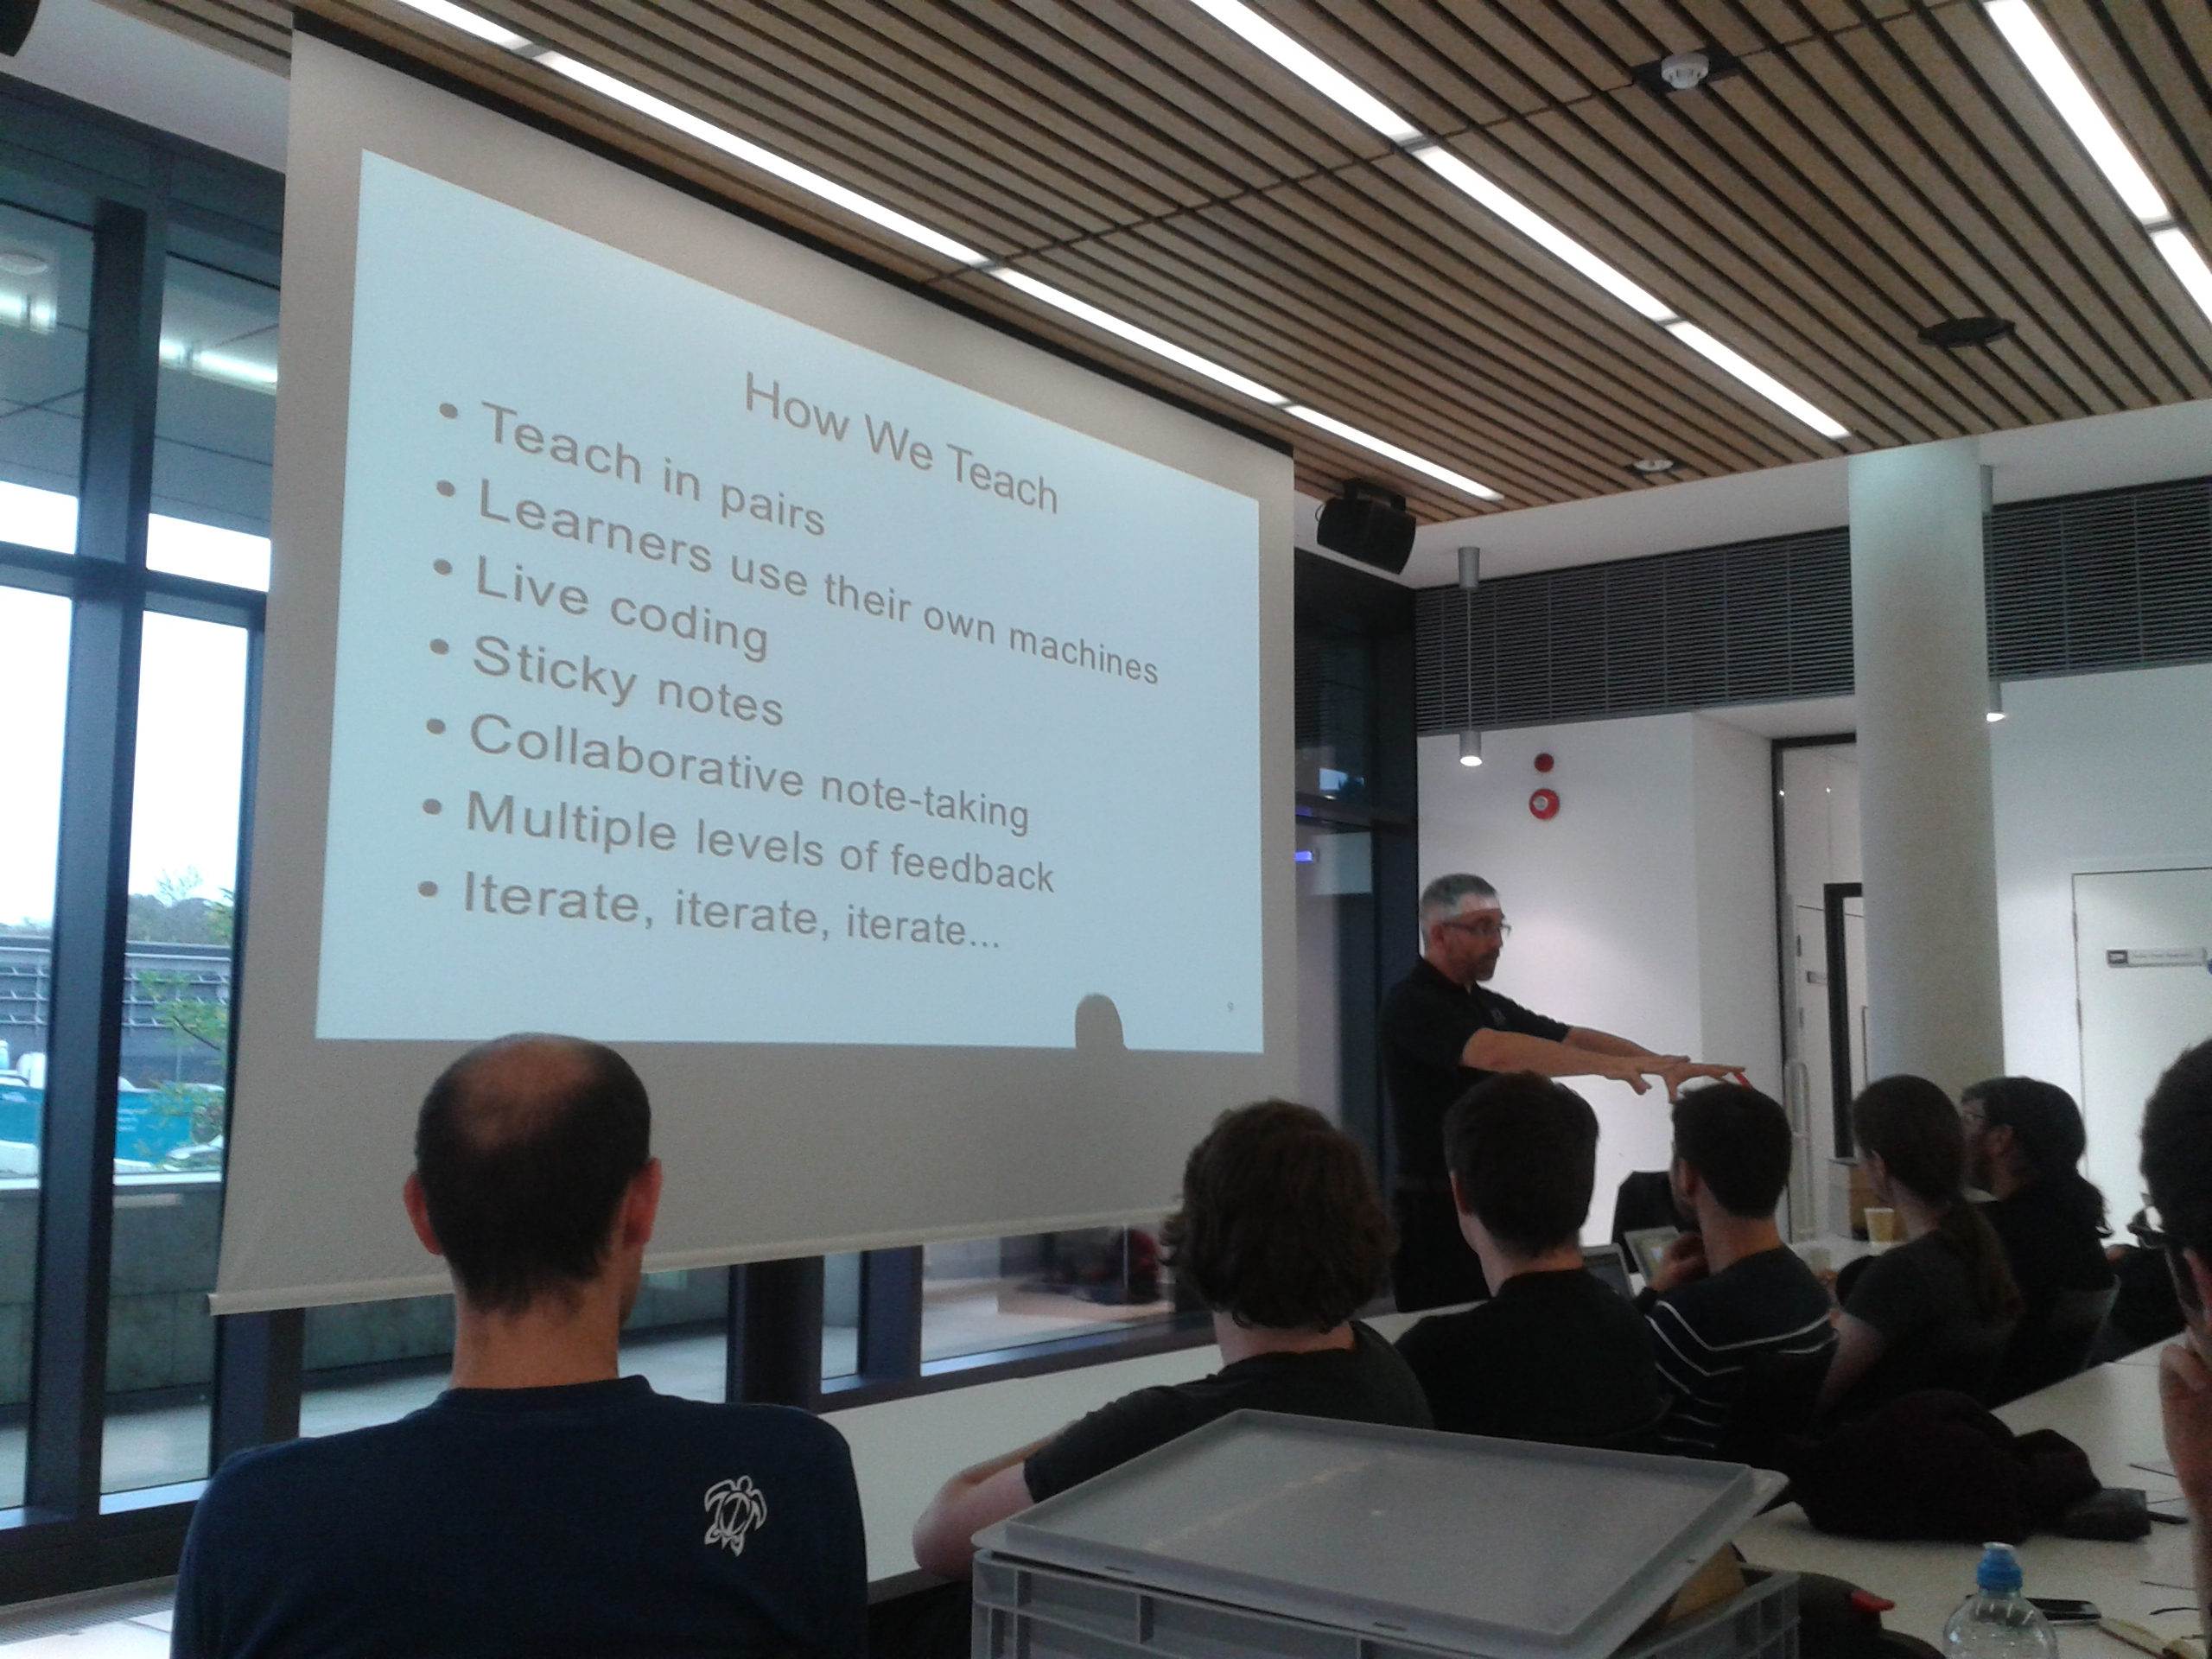
\includegraphics[width=8in]{ian-2015-11-10-Greg-Wilson.jpg}
\caption*{\textit{Greg mind-melds with a future instructor}}
\end{figure}
\vspace{-0.25cm}

In one amazing visit by Greg he gave me and our group of students loads of
ideas and enthusiasm, and then found time to talk me through a problem I had
with an ex-advisee. Above all he's given me the confidence to try something,
fail well, and then get back up and try again.

\signed{Ian Hawke}

\newpage

{\LARGE Technical Details}

The basic template for this book was put together by Eric Jeschke in
2009, as part of a ``Solo Photo Book Month'' project.  The original book
is titled \title{Chickens, Anyone?} and is a lovely recounting of his
family's adventures with raising chickens in their back yard.  The template
was pointed out to me (Erik) by Jonah Duckles, and by complete coincidence
I am personally acquainted with Eric Jeschke, and knowing of his talent I
immediately decided to adopt his work as my template, as he has made it
freely available for copying:

https://redskiesatnight.com/books/pod/latex-templates-for-pod-publishing-with-blurb-com

You'll note that much of the layout of the book was inspired by his book,
so credit where credit is due.

I did what I could with photos taken off the web, and some sent to me by
individual respondents.  Many of them will not be,
perfectionalistically-speaking, `print-quality', but they'll have to do given
that this was done on short time.

The book is written using \LaTeX with {\em xetex} and {\em xdvipdfmx} for
easier adjustments for dead tree publishing.  The font used is EB Garamond.
The book was made on Cygwin, and files were tracked in (I'm sorry to say) a
{\em git} repository.  As we were short on time it did not follow many good
software development practices such as reuse or scripting of repetitive tasks
due in part to xkcd\#1319:
\begin{figure}[h!]
\centering
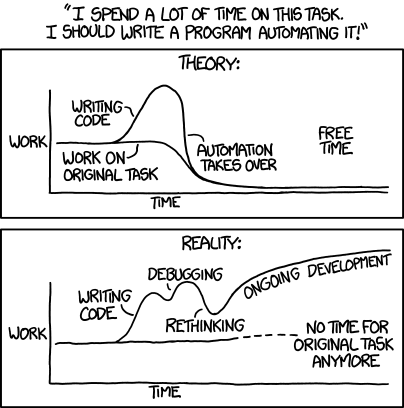
\includegraphics[width=4in]{automation}
\end{figure}

%END


\end{document}
